In this chapter we review the results obtained through out this work and obtain phyisicaly relevant quantities from our simulations and analytical computations.

\section{Comparing Numeric An Analytic Results In Steady State Regime}

Fig. \ref{fig:comparison} shows the comparison between the numeric and analytic results. 



\begin{figure}[htbp]
\begin{subfigure}{.5\linewidth}
\centering
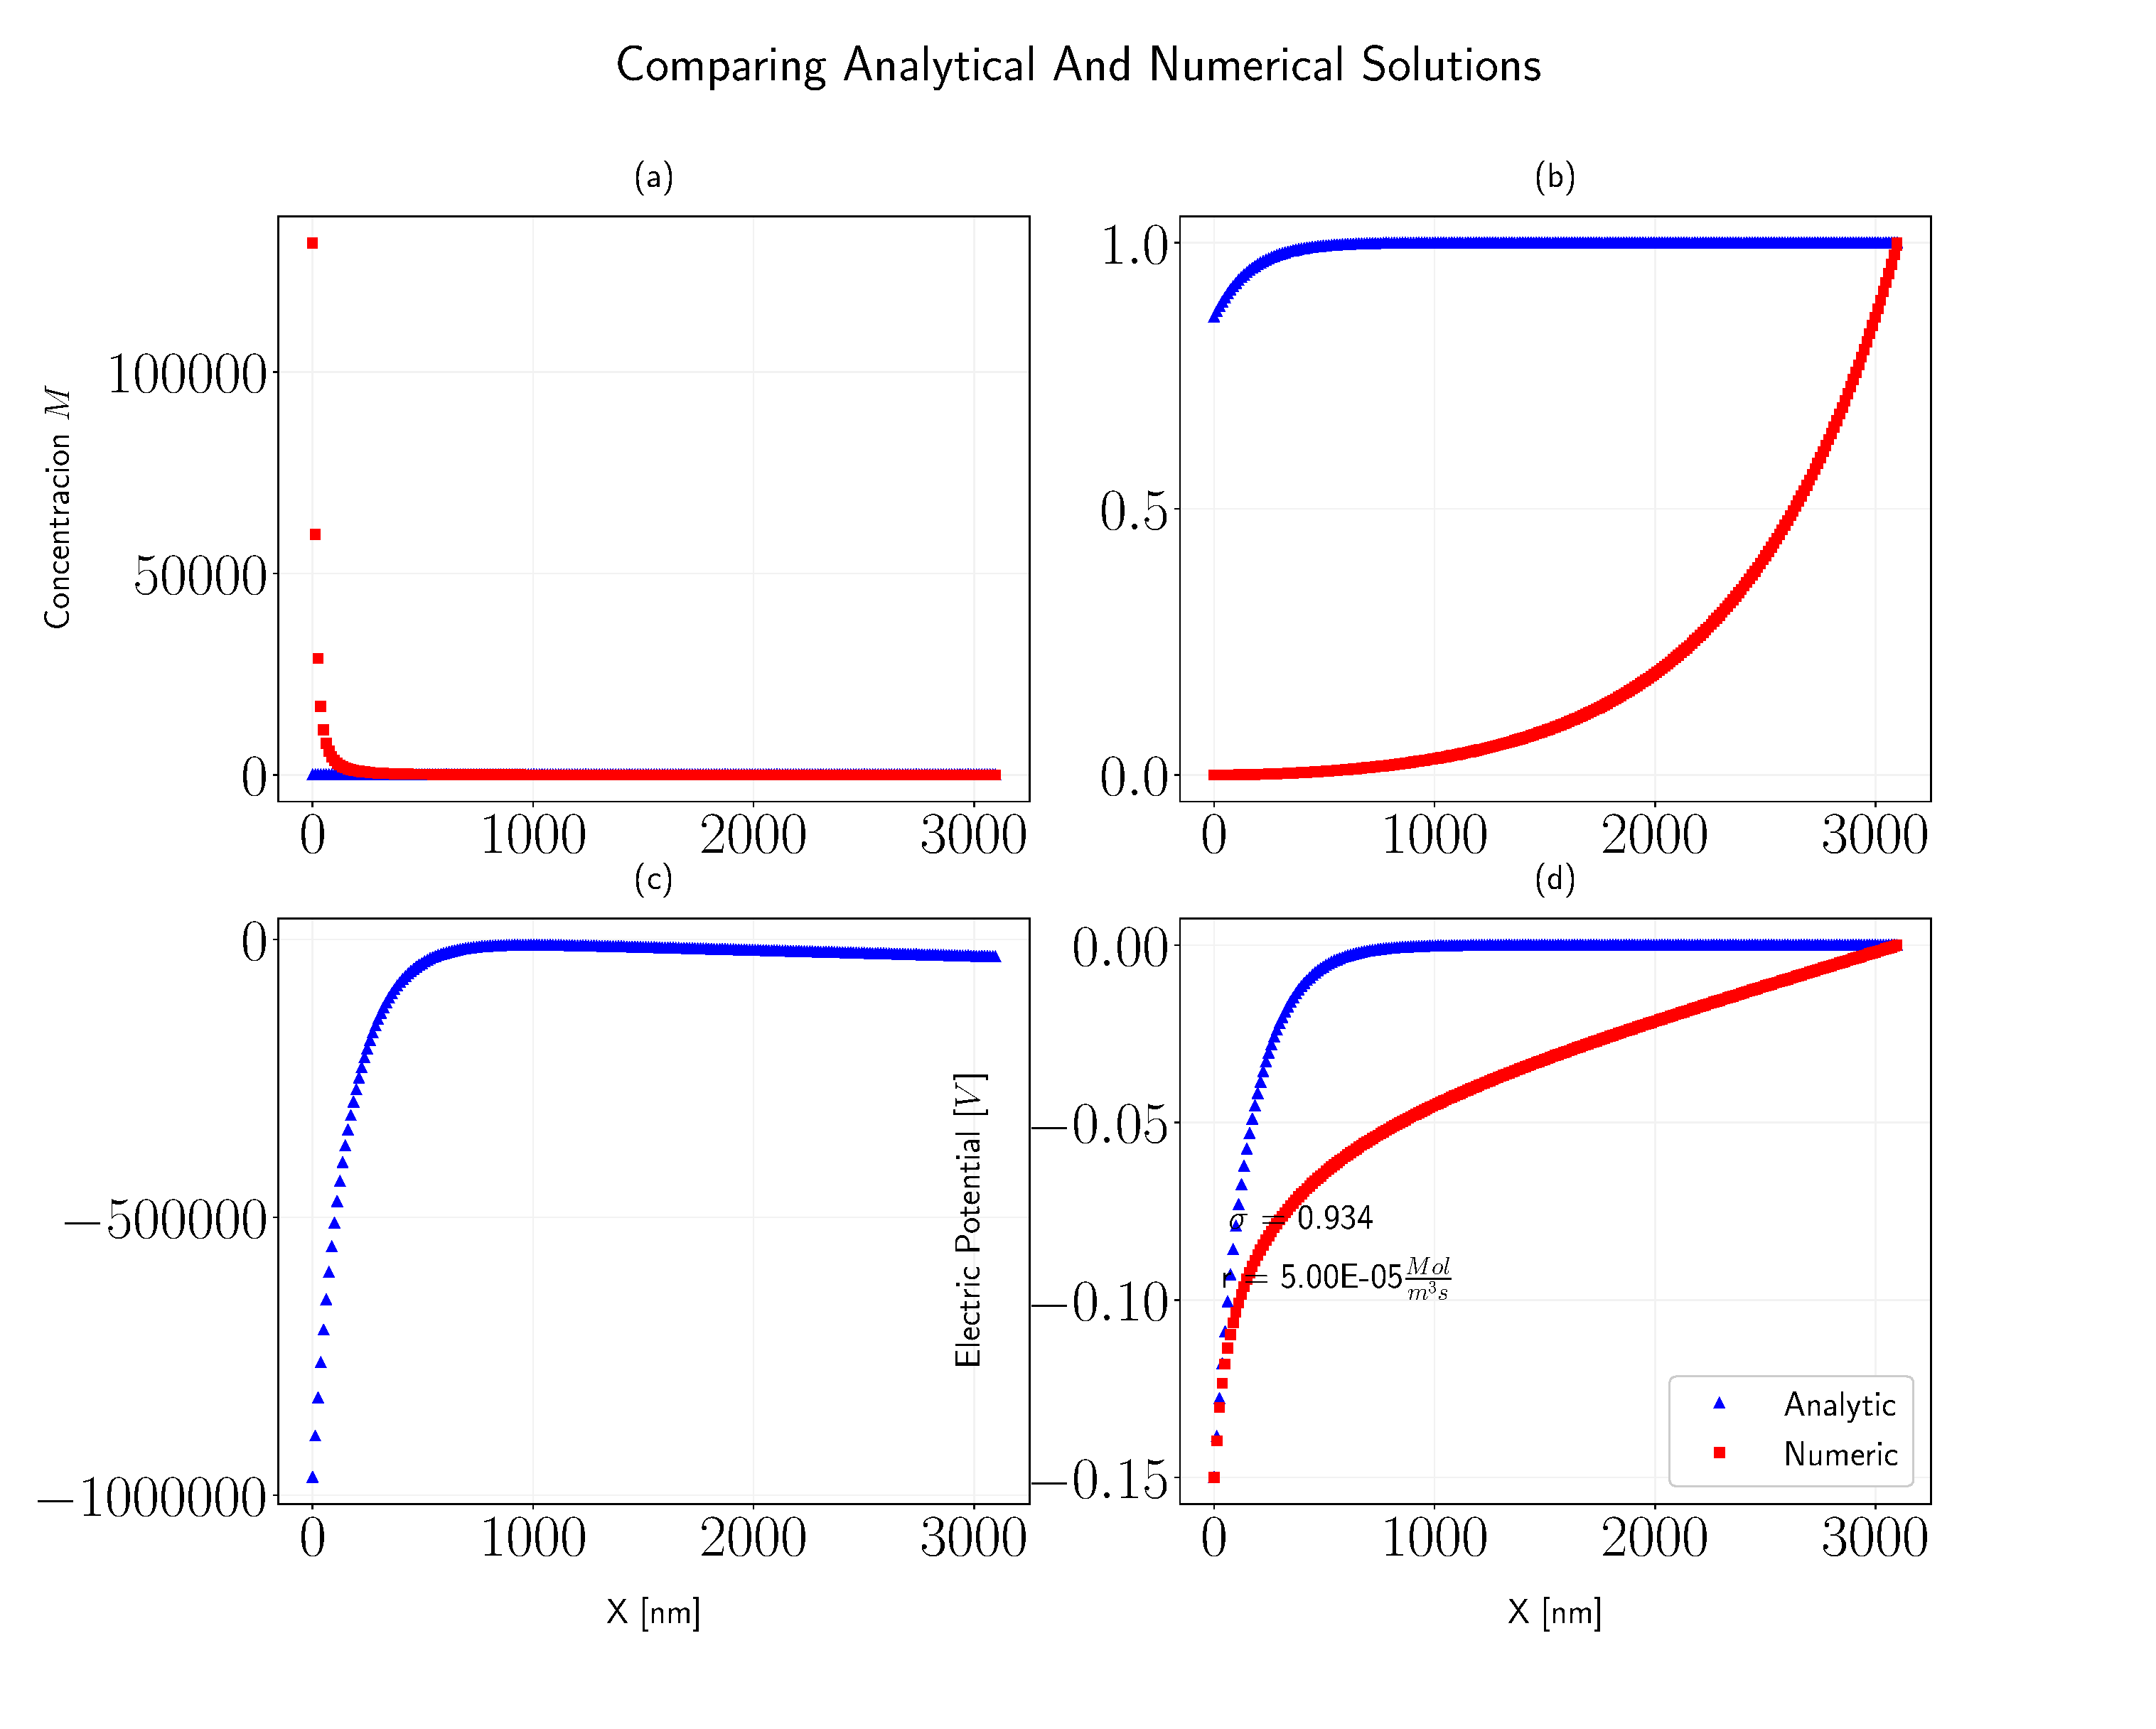
\includegraphics[width=\textwidth]{comparison0}
\caption{}
\label{fig:sub1}
\end{subfigure}%
\begin{subfigure}{.5\linewidth}
\centering
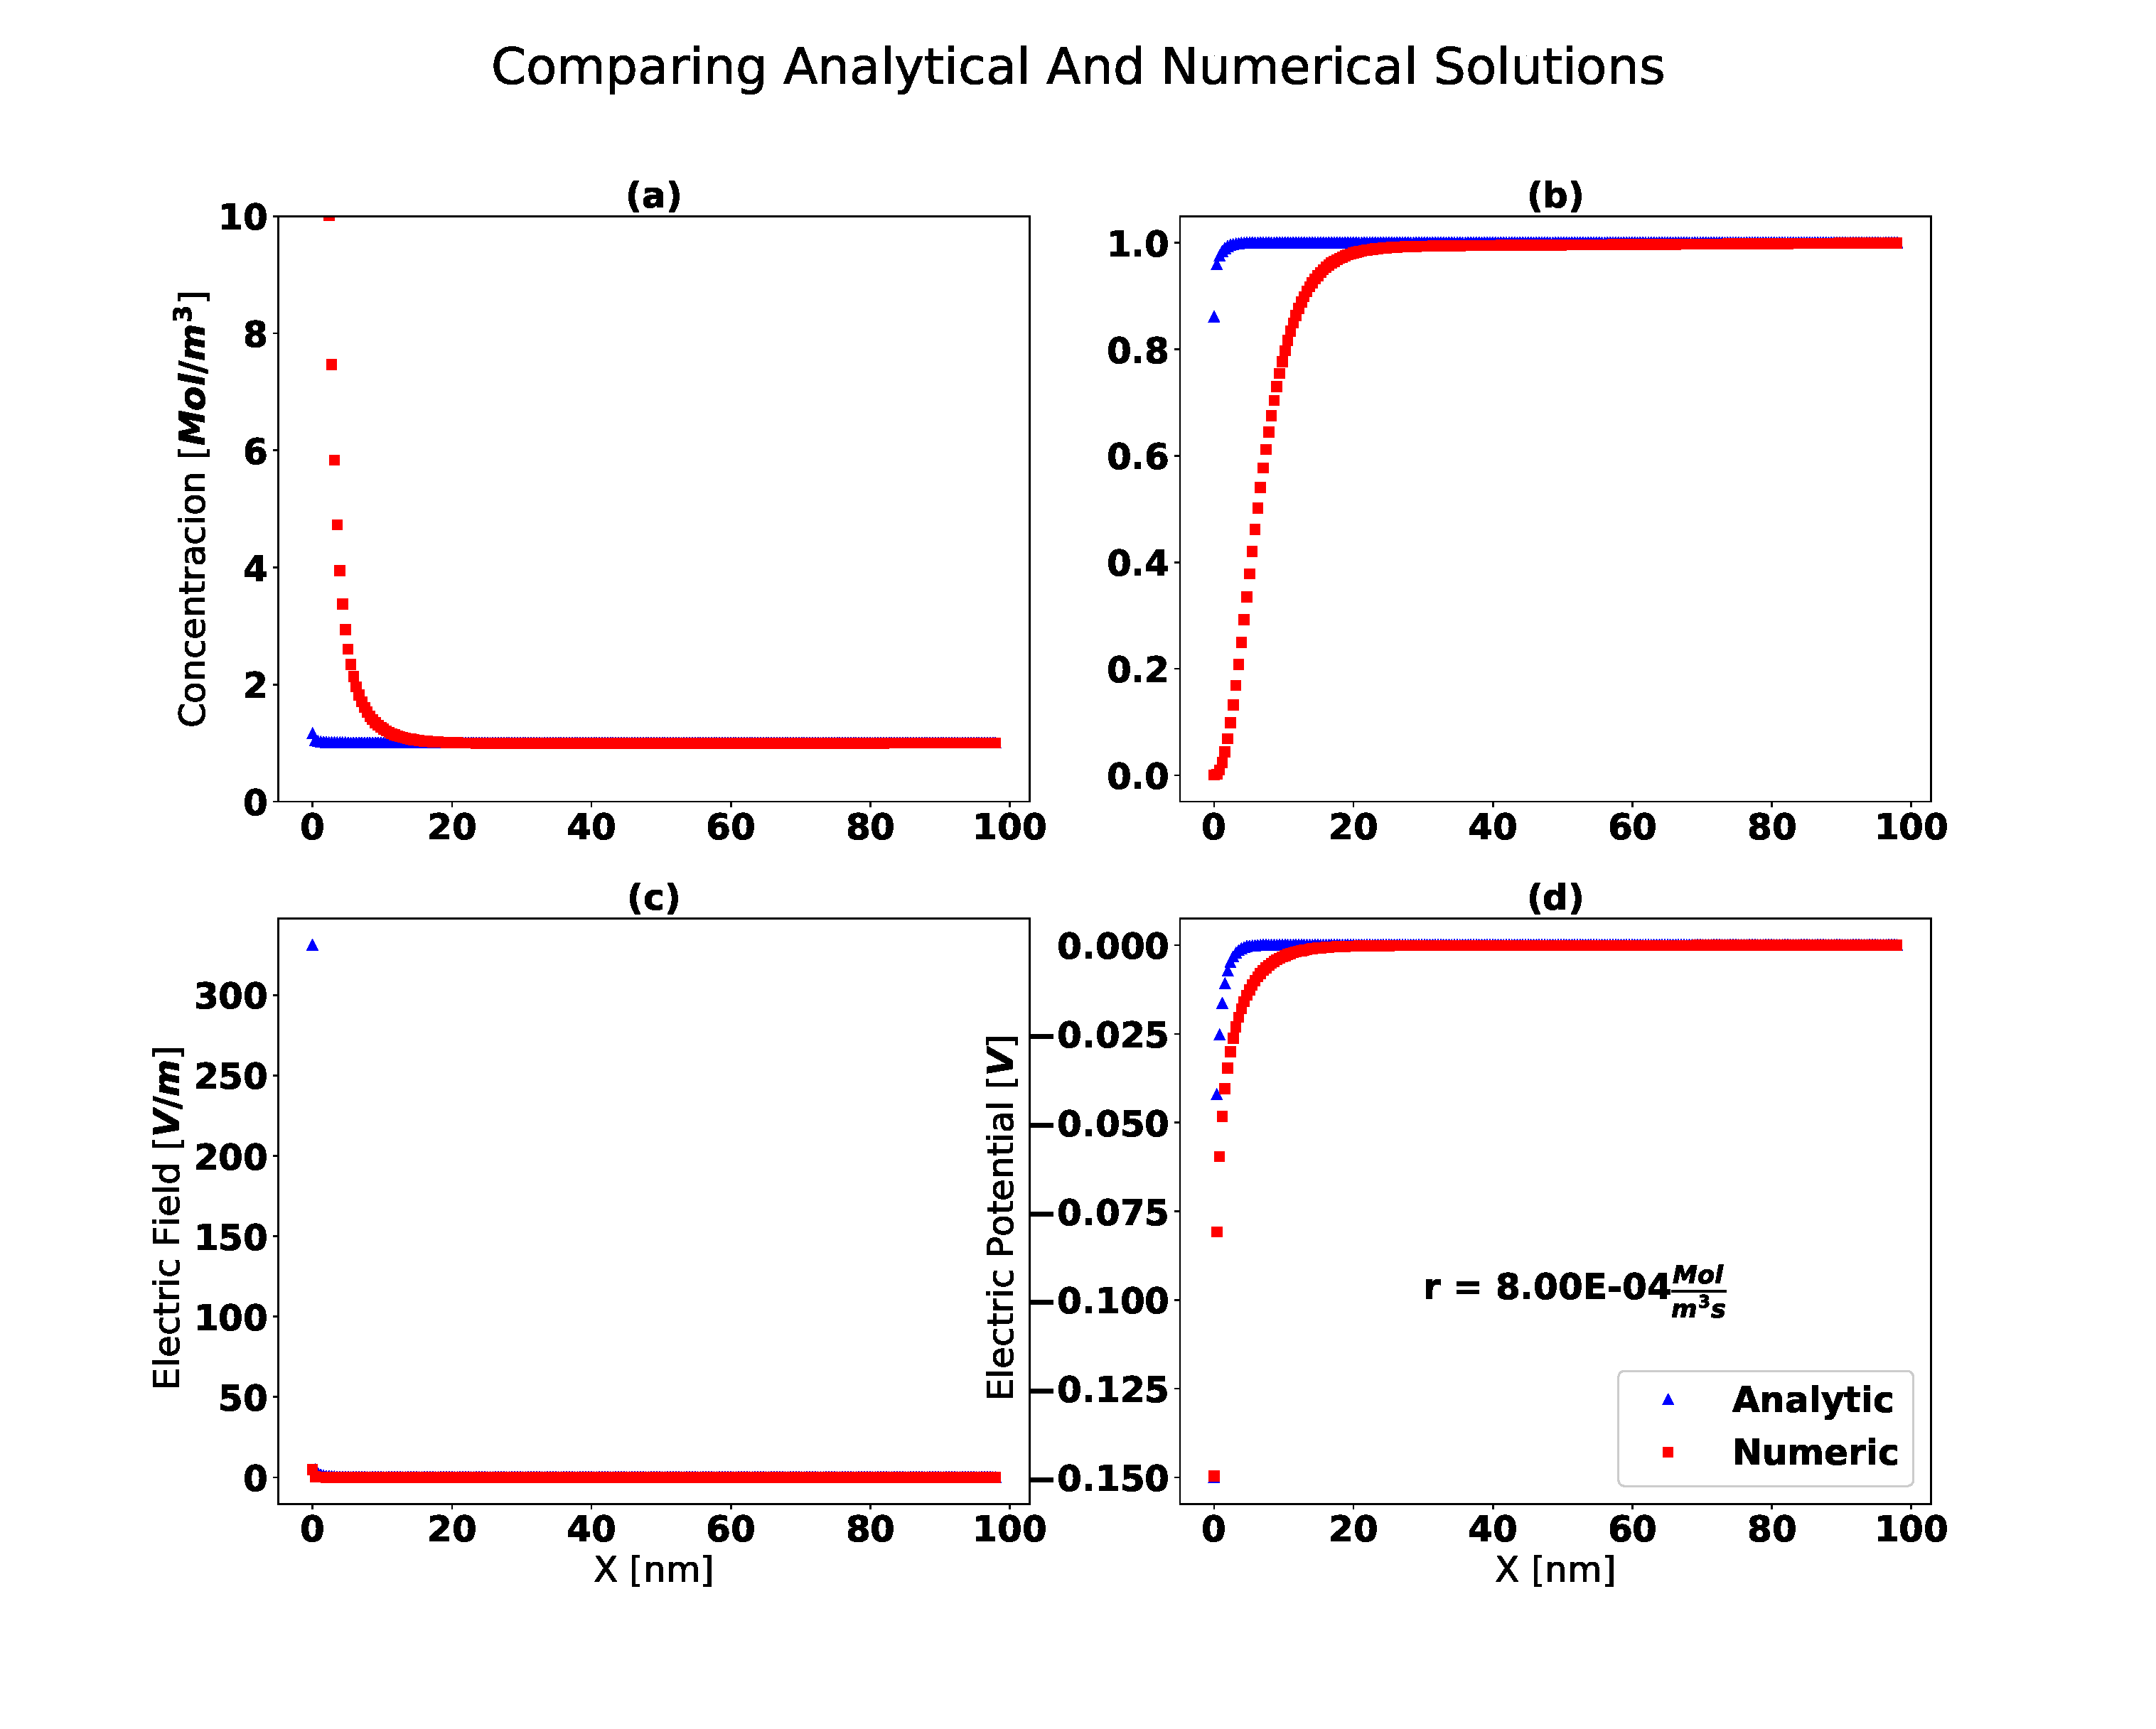
\includegraphics[width =\textwidth]{comparison1}
\caption{}
\label{fig:sub2}
\end{subfigure}\\[1ex]
\begin{subfigure}{\linewidth}
\centering
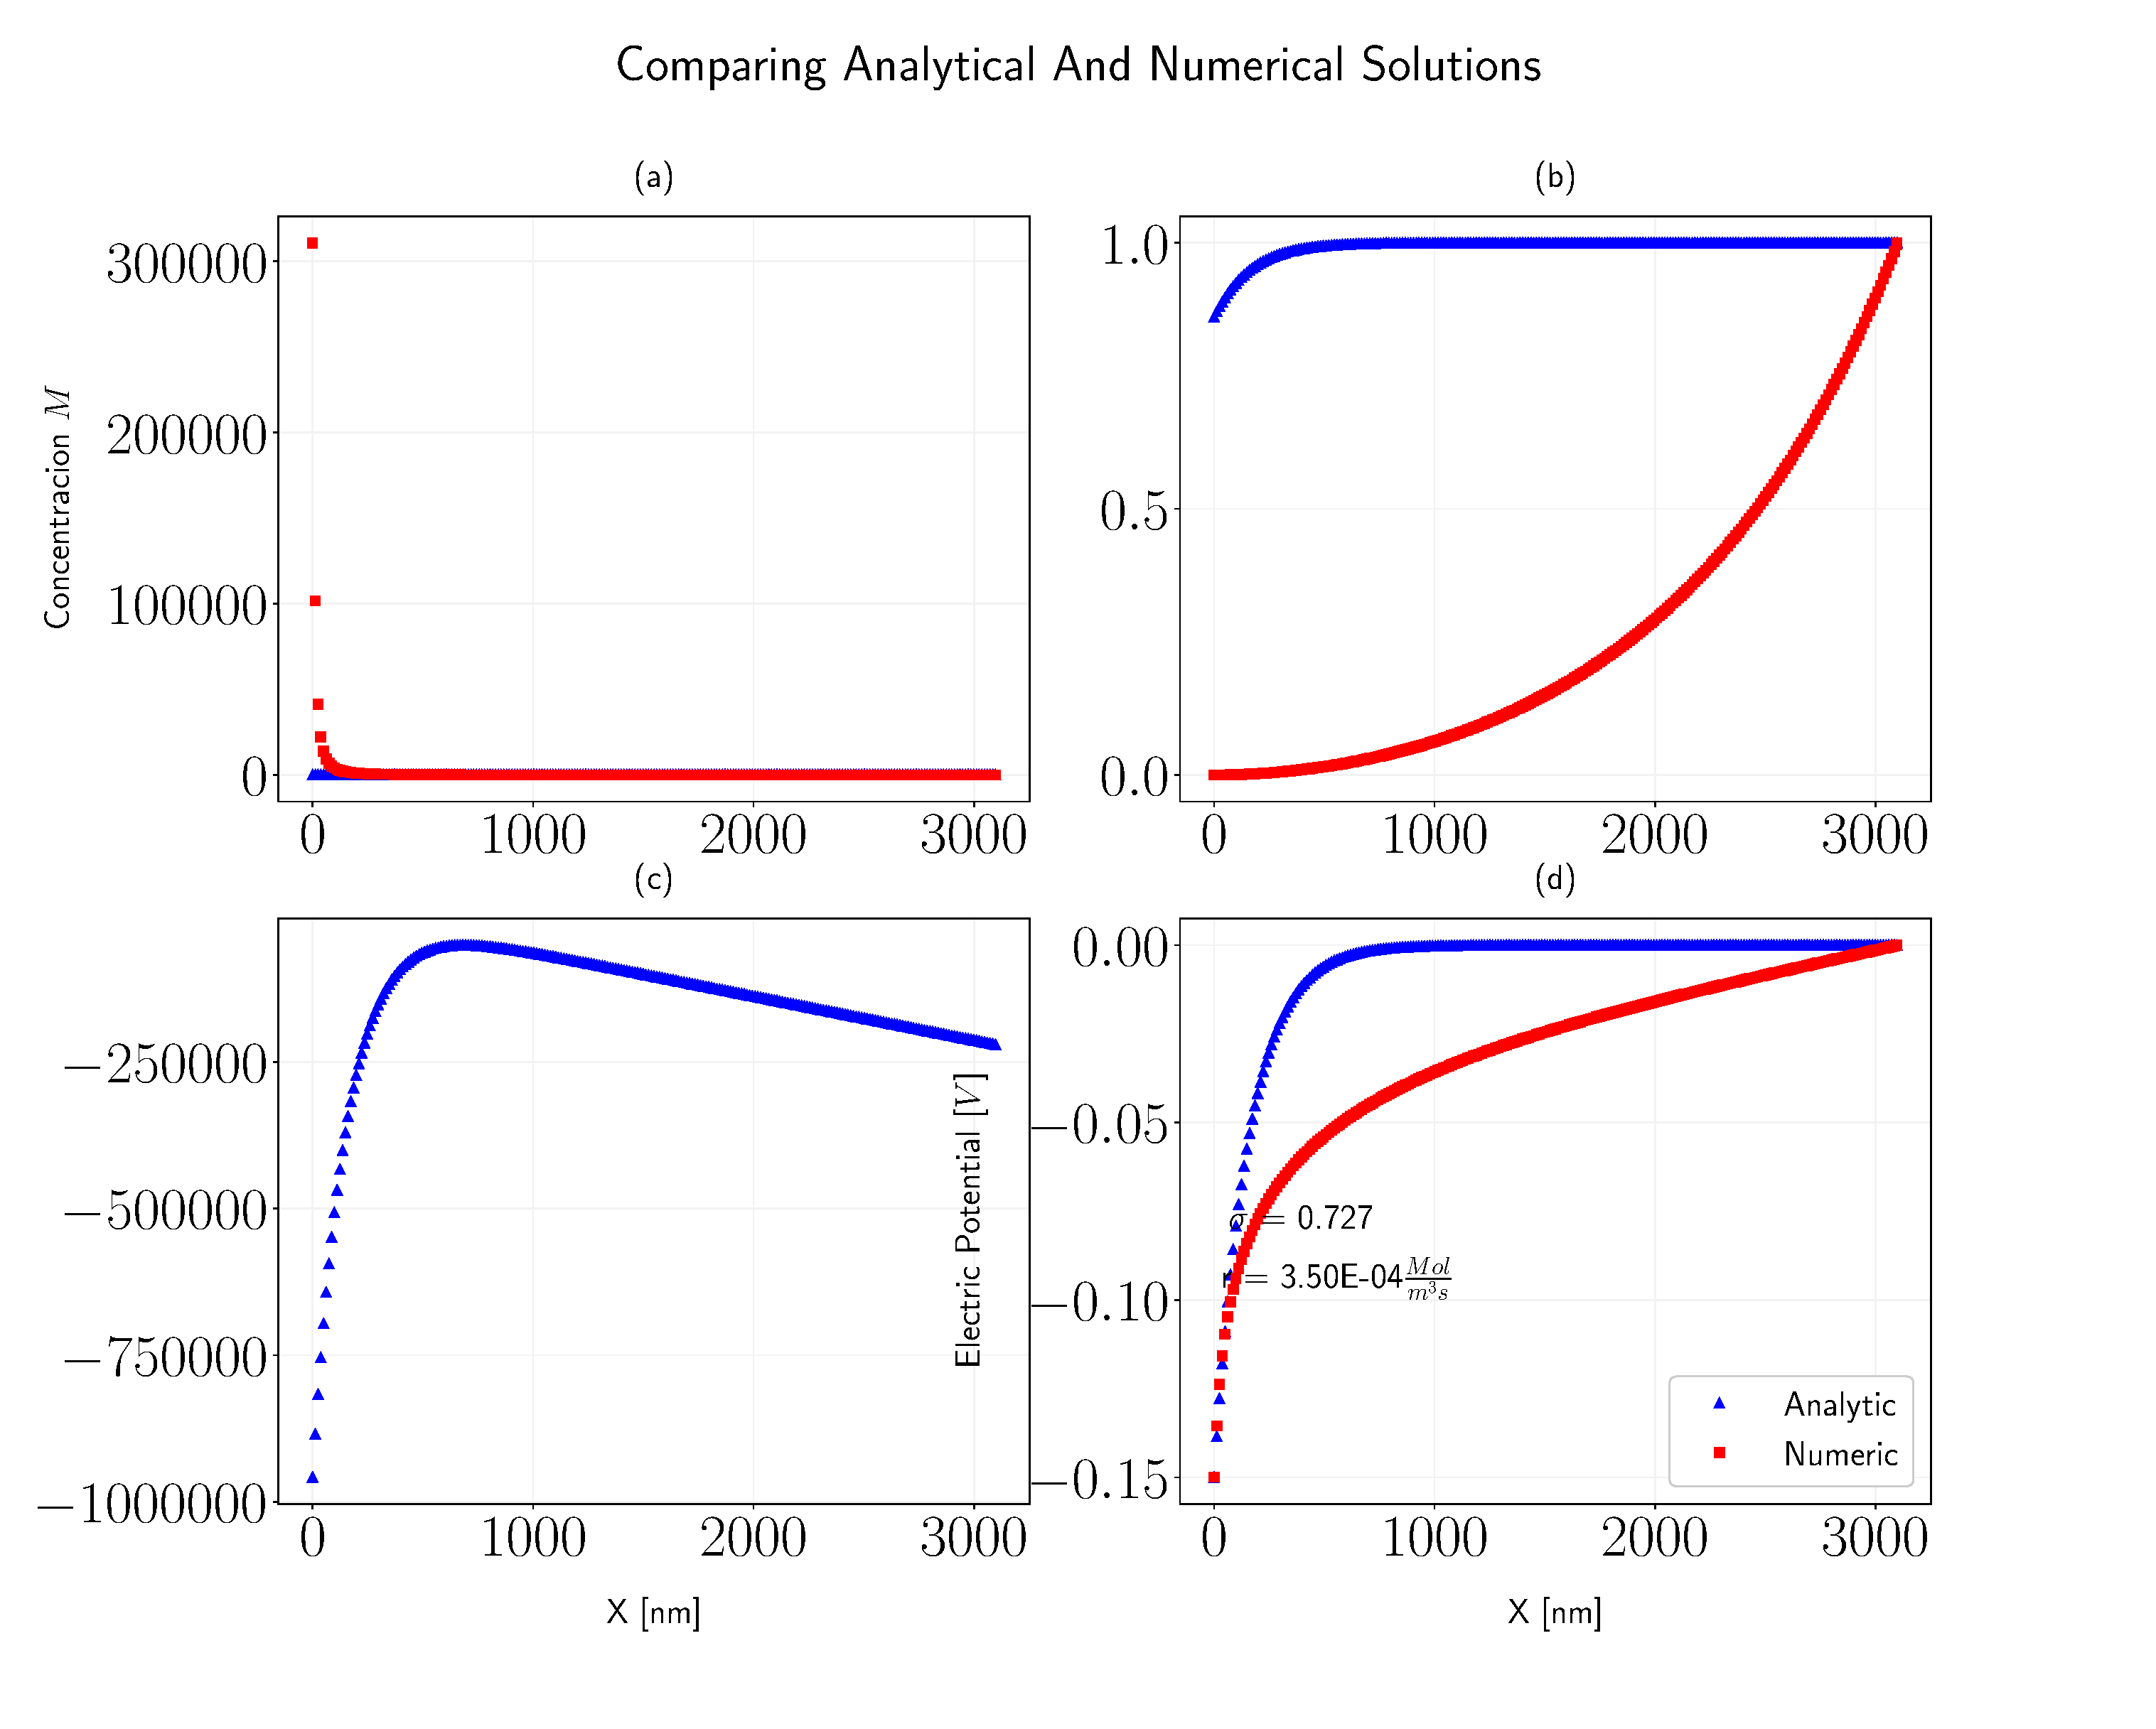
\includegraphics[width =0.5\textwidth]{comparison2}
\caption{}
\label{fig:sub3}
\end{subfigure}
\caption{Three subfigures}
\label{fig:test}
\end{figure}


\newpage

